% Provenance (never printed): see sources/outline_sources.md (Year 3:
% energy-balance models, the one-layer model recalled; ice-albedo feedback
% and multiple equilibria; how general circulation models are built and
% evaluated).
% Brief: sources/book5/BRIEFS.md, ch. 22. Curves from
% figdata/bachelor-3/budyko_sellers.py (the zero-dimensional model and
% Budyko's latitudinal model; the brief's ebm_0d is folded into it) and
% two_layer.py. Exercise and problem values in the Book 5 scratch calculator
% calc/ch22.py. The model planet, model X and the ensemble of exercise 12 are
% invented.
\chapter{Modelos climáticos}\label{ch:b3:climate-models}

Se toma la radiación solar que llega a la Tierra, \qty{340}{W/m^2} promediada sobre
el globo y una ley para el infrarrojo que devuelve al espacio, ajustada a
treinta años de un reanálisis de las observaciones. El albedo del planeta crece desde el de
suelo desnudo y mar hasta el del hielo a medida que la superficie se enfría. Se igualan los dos
flujos, y la ecuación tiene tres soluciones: un planeta a
\qty{14}{\celsius}, cercana a la media del planeta real; un planeta a
\qty{8}{\celsius}; y un planeta a \qty{-46}{\celsius}, congelado de polo a
polo. Los modelos climáticos, desde estas pocas líneas hasta los programas que se ejecutan en las
computadoras más grandes, son herramientas para preguntar qué clima tiene un planeta dado, cómo
llega a él y cómo cambia cuando se perturba su balance energético.
% ledger: nasa:solar-mean, data:b5-ncep-air, data:b3-ncep, budyko69:albedo

\begin{recall}
El cuerpo negro, la ley de Stefan--Boltzmann, el efecto invernadero y el
modelo de una capa de la atmósfera están en los libros de física; el albedo y el
balance energético de la Tierra, en los libros escolares. La radiación de onda larga
saliente, la temperatura de emisión y el transporte meridional de calor están en el
volumen de primer año, en su capítulo sobre radiación y transporte de calor.
La retroalimentación hielo--albedo y la Tierra bola de nieve están en el volumen de segundo año, en
su capítulo sobre la Tierra precámbrica; el forzamiento radiativo efectivo, el
parámetro de retroalimentación climática $\lambda < 0$, la sensibilidad climática de
equilibrio (ECS, por sus siglas en inglés) y la respuesta climática transitoria (TCR, por sus siglas en inglés) en su capítulo
sobre el cambio climático antropogénico; la predicción numérica del tiempo y la
predicción por conjuntos en su capítulo sobre sistemas meteorológicos. Las ecuaciones de
movimiento en la Tierra en rotación, con la \omterm{def:b3:gfd-foundations:hydrostatic}{aproximación hidrostática}, están en
el capítulo~\ref{ch:b3:gfd-foundations}.
\end{recall}

\section{El balance energético de un planeta}\label{sec:b3:climate-models:zero-d}

Promediado sobre la esfera y sobre un año, cada metro cuadrado en el tope de
la atmósfera recibe $Q = S_0/4 = \qty{340}{W/m^2}$, una cuarta parte de la
irradiancia solar $S_0 = \qty{1360}{W/m^2}$. Una fracción $\alpha$, el
albedo planetario, se refleja; el resto, $Q(1 - \alpha)$, se absorbe y
debe devolverse al espacio como infrarrojo. Un cuerpo negro emitiría $\sigma
T^4$; la radiación de onda larga saliente de la Tierra (OLR, por sus siglas en inglés) es menor, debido al
efecto invernadero, y en el intervalo de temperaturas superficiales que se encuentran en
la Tierra es casi una línea recta,
\[
\text{OLR} = A + BT ,
\]
con $T$ la temperatura superficial en grados Celsius. En 1969 Budyko ajustó
una ley de este tipo a la radiación saliente calculada en 260 estaciones, con una corrección por
nubosidad $n$: $I = a + bT - (a_1 + b_1T)n$, $a = 14.0$, $b = 0.14$, $a_1 =
3.0$ y $b_1 = 0.10$ en \unit{kcal.cm^{-2}} por mes, con una dispersión inferior a
\qty{5}{\percent}. Para una nubosidad media de 0.5 se obtiene $A =
\qty{199}{W/m^2}$ y $B = \qty{1.43}{W.m^{-2}.\celsius^{-1}}$. Las
\omterm{def:b3:atmospheric-dynamics:eddy}{medias zonales} anuales de la NCEP--NCAR Reanalysis~1 para 1991--2020, ponderadas por área,
dan $A = \qty{211.9}{W/m^2}$ y $B = \qty{1.816}{W.m^{-2}.\celsius^{-1}}$,
con una dispersión de \qty{10}{W/m^2} alrededor de la recta. Estos valores se
emplean a continuación.
% ledger: nasa:solar-mean, budyko69:olr, data:b5-ncep-air, data:b3-ncep

\begin{definition}[Modelo de balance energético]\label{def:b3:climate-models:ebm}
Un \emph{modelo de balance energético}\index{modelo de balance energético} es un
modelo climático que calcula una temperatura superficial --- una única media global, o una
media sobre cada latitud --- a partir del balance de la radiación solar absorbida, la
radiación infrarroja emitida al espacio y, si la temperatura depende de la latitud, el
calor transportado hacia los polos. En su forma de dimensión cero,
\[
C\,\frac{\mathrm dT}{\mathrm dt} = Q\big(1 - \alpha(T)\big) - (A + BT) ,
\]
donde $C$ es la capacidad calorífica por unidad de área de la parte del sistema que
se calienta junto con la superficie.
\end{definition}

Con $\alpha = 0.30$, el equilibrio es $T = (238 - 211.9)/1.816 =
\qty{14.4}{\celsius}$; la media ponderada por área del reanálisis es
\qty{14.2}{\celsius}. Un forzamiento $F$, como el de un cambio del
dióxido de carbono, se suma al miembro derecho. Cerca de un equilibrio la respuesta está
gobernada por el parámetro de retroalimentación climática $\lambda$ del volumen de segundo año:
con el albedo fijo, $\lambda = -B$.
% ledger: earth:albedo, data:b5-ncep-air

\begin{theorem}[Tiempo de respuesta de un clima de una sola caja]\label{thm:b3:climate-models:response}
Sea un clima en equilibrio, y sea un forzamiento constante $F$ que se active
en $t = 0$. Si la desviación $T'$ respecto del equilibrio obedece $C\,\mathrm
dT'/\mathrm dt = F + \lambda T'$ con $C > 0$ y $\lambda < 0$ constantes,
entonces
\[
T'(t) = -\frac{F}{\lambda}\Big(1 - \mathrm e^{-t/\tau}\Big), \qquad
\tau = -\frac{C}{\lambda} .
\]
El nuevo equilibrio es $-F/\lambda$, y el clima recorre la fracción $1
- \mathrm e^{-1} = \num{0.63}$ del camino en el tiempo $\tau$.
\end{theorem}

\begin{proof}
$T'_\infty = -F/\lambda$ anula el miembro derecho. La diferencia
$u = T' - T'_\infty$ obedece $C\,\mathrm du/\mathrm dt = \lambda u$, por lo que $u =
u(0)\,\mathrm e^{\lambda t/C}$, con $u(0) = F/\lambda$.
\end{proof}

La capacidad calorífica que importa en unos pocos años es la del océano superior.
El emulador de dos capas del sexto informe de evaluación del
Grupo Intergubernamental de Expertos sobre el Cambio Climático, calibrado con 44 modelos climáticos,
proporciona para la capa superficial $C = \qty{8.1}{W.yr.m^{-2}.\celsius^{-1}}$, la
capacidad calorífica de una capa de agua de mar de \qty{62}{m} de profundidad. Con $\lambda = -B$ el
tiempo de respuesta es $8.1/1.816 = \num{4.5}\text{ años}$. El clima real también calienta
el océano profundo, mucho más lentamente; la sección~\ref{sec:b3:climate-models:two-layer}
lo incorpora.
% ledger: ar6sm7:two-layer, teos10:cp0, data:b5-ncep-air

\section{Hielo, albedo y equilibrios múltiples}\label{sec:b3:climate-models:multiple}

La retroalimentación hielo--albedo del volumen de segundo año hace que el albedo dependa de
la temperatura. Se toma $\alpha = 0.62$ para un planeta cuya superficie esté por debajo de
$T_I = \qty{-10}{\celsius}$, el albedo del hielo en el modelo de Budyko, $\alpha
= 0.30$ por encima de $T_F = \qty{+10}{\celsius}$, y una recta entre ambos valores, a medida que
el hielo retrocede. La rampa es una elección de este capítulo; cualquier albedo que
aumente a medida que el planeta se enfría produce el mismo cuadro.
% ledger: budyko69:albedo, earth:albedo

\begin{definition}[Equilibrios climáticos múltiples; bifurcación silla-nodo]\label{def:b3:climate-models:multiple-equilibria}
Un modelo climático tiene \emph{equilibrios climáticos múltiples}\index{equilibrios climáticos múltiples}
cuando, para las mismas condiciones externas, tiene más
de un estado estacionario. Un equilibrio es estable si una pequeña desviación respecto
de él decae, e inestable si crece. Una \emph{bifurcación
silla-nodo}\index{bifurcación silla-nodo} es el valor de un parámetro en el que
un equilibrio estable y uno inestable se encuentran y desaparecen juntos.
\end{definition}

\begin{proposition}[Tres equilibrios y su estabilidad]\label{prop:b3:climate-models:three}
Se escribe $N(T) = Q(1 - \alpha(T)) - (A + BT)$ para el flujo neto descendente. Un
equilibrio $T^*$, $N(T^*) = 0$, es estable si $N'(T^*) < 0$ e inestable si
$N'(T^*) > 0$. Con la rampa anterior, $N' = -B$ en las ramas de bola de nieve y
sin hielo, que son estables allí donde existen, y $N' = -B -
Q\,\mathrm d\alpha/\mathrm dT$ en la rampa, que es inestable cuando $Q\,
|\mathrm d\alpha/\mathrm dT| > B$. Para $Q = \qty{340}{W/m^2}$ el modelo tiene
tres equilibrios, \qty{-45.5}{\celsius} (estable), \qty{7.8}{\celsius}
(inestable) y \qty{14.4}{\celsius} (estable).
\end{proposition}

\begin{proof}
Cerca de $T^*$, $C\,\mathrm dT'/\mathrm dt = N'(T^*)T'$, que decae si
$N'(T^*) < 0$ y crece si $N'(T^*) > 0$. En la rampa $\mathrm d\alpha/
\mathrm dT = -0.32/20 = \qty{-0.016}{\celsius^{-1}}$, así que $N' = -1.816 + 340
\times 0.016 = \qty{+3.62}{W.m^{-2}.\celsius^{-1}}$. La rama de bola de nieve,
$T = (340\times0.38 - 211.9)/1.816 = \qty{-45.5}{\celsius}$, queda por debajo de
$T_I$; la cálida, \qty{14.4}{\celsius}, por encima de $T_F$; en la rampa,
$340(0.54 + 0.016\,T) = 211.9 + 1.816\,T$ da $T = \qty{7.8}{\celsius}$.
\end{proof}

\begin{omfigure}
\begin{tikzpicture}
\begin{groupplot}[group style={group size=2 by 1, horizontal sep=1.5cm},
  width=0.48\linewidth, height=0.4\linewidth,
  tick label style={font=\scriptsize}, label style={font=\small}, title style={font=\small}]
\nextgroupplot[xlabel={$T$ (\unit{\celsius})}, ylabel={flujo (\unit{W/m^2})},
  xmin=-60, xmax=40, ymin=80, ymax=270, title={balance para $Q = \qty{340}{W/m^2}$},
  legend style={font=\scriptsize, at={(0.03,0.97)}, anchor=north west}]
% computed in figdata/bachelor-3/budyko_sellers.py
\addplot[omThm, thick] table[x=T, y=asr] {figdata/out/bachelor-3-budyko_sellers-asr.dat};
\addlegendentry{luz solar absorbida}
\addplot[omDef, thick] table[x=T, y=olr] {figdata/out/bachelor-3-budyko_sellers-olr.dat};
\addlegendentry{$A + BT$}
\addplot[only marks, mark=*, mark size=2pt, forget plot] coordinates {(-45.55,129.2) (14.38,238.0)};
\addplot[only marks, mark=o, mark size=2pt, thick, forget plot] coordinates {(7.81,226.07)};
\node[font=\scriptsize, anchor=north west] at (axis cs:-45.55,125) {bola de nieve};
\draw[black!60] (axis cs:7.81,226.07) -- (axis cs:16,200);
\node[font=\scriptsize, anchor=north west, inner sep=1pt] at (axis cs:16,200) {inestable};
\nextgroupplot[xlabel={$S_0$ (\unit{W/m^2})}, ylabel={$T$ (\unit{\celsius})},
  xmin=1000, xmax=2200, ymin=-70, ymax=100, title={equilibrios e histéresis},
  scaled x ticks=false, xticklabel style={/pgf/number format/1000 sep={}}]
\addplot[black!40, densely dotted, forget plot] coordinates {(1360,-70) (1360,100)};
\addplot[omMeth, thick] table[x=S, y=T] {figdata/out/bachelor-3-budyko_sellers-eqwarm.dat};
\addplot[omThm, thick] table[x=S, y=T] {figdata/out/bachelor-3-budyko_sellers-eqcold.dat};
\addplot[black!60, thick, dashed] table[x=S, y=T] {figdata/out/bachelor-3-budyko_sellers-eqmid.dat};
\draw[->, thick, black!70] (axis cs:1314.6,8) -- (axis cs:1314.6,-45);
\draw[->, thick, black!70] (axis cs:2039.4,-8) -- (axis cs:2039.4,77);
\node[font=\scriptsize, anchor=south, black!60, fill=white, inner sep=1pt] at (axis cs:1360,84) {hoy};
\node[font=\scriptsize, omMeth, anchor=north west] at (axis cs:1700,32) {cálida};
\node[font=\scriptsize, omThm, anchor=north] at (axis cs:1620,-40) {bola de nieve};
\end{groupplot}
\end{tikzpicture}

\par\smallskip{\small El \omterm{def:b3:climate-models:ebm}{modelo de balance energético} de dimensión cero con una
rampa hielo--albedo y la ley de OLR ajustada a la Reanalysis~1 de NCEP--NCAR.
A la izquierda, la luz solar absorbida y el infrarrojo emitido para la luz solar de hoy:
se cruzan tres veces; los círculos rellenos son estables y el abierto es inestable.
A la derecha, la temperatura de equilibrio frente a la constante solar, con las ramas estables
en línea continua y la inestable en discontinua. Al disminuir la radiación solar desde el
valor de hoy enfría el planeta cálido hasta que la rama cálida termina en
\qty{1315}{W/m^2}, y el clima cae en la bola de nieve; permanece congelado
hasta que la radiación solar se eleva a \qty{2039}{W/m^2}, donde salta de nuevo a un
planeta muy caliente, muy por encima del intervalo en el que la OLR lineal
es válida.}\label{fig:b3:climate-models:zero-d}
\end{omfigure}
% ledger: nasa:solar-mean, data:b5-ncep-air, budyko69:albedo, earth:albedo

A medida que $Q$ disminuye, el equilibrio cálido se enfría y el equilibrio de la rampa se calienta.
Se encuentran en lo alto de la rampa, $T = T_F$, donde $Q(1 - 0.30) = A +
10B$: $Q = \qty{328.7}{W/m^2}$, lo que da una constante solar de \qty{1315}{W/m^2},
\qty{3.3}{\percent} por debajo de la de hoy. Se trata de una \omterm{def:b3:climate-models:multiple-equilibria}{bifurcación silla-nodo}: por debajo
de ella el único equilibrio es la bola de nieve, y el clima cae en ella.
Volver a elevar la radiación solar no devuelve el planeta cálido: la rama de bola de nieve
termina solo donde su temperatura alcanza $T_I$, $Q(1 - 0.62) = A -
10B$, con una constante solar de \qty{2039}{W/m^2}, \qty{50}{\percent} por encima
de la de hoy. Entre ambas, el estado del planeta depende de su historia:
el modelo presenta histéresis. En el Neoproterozoico real, la salida de la
bola de nieve del volumen de segundo año no fue un Sol más brillante, sino el dióxido de carbono
de los volcanes, acumulado durante millones de años hasta que el
forzamiento de efecto invernadero alcanzó el umbral de deglaciación; la línea de hielo retrocedió entonces hasta
los polos en unos pocos miles de años.
% ledger: hoffman17:hysteresis

\section{El modelo de Budyko--Sellers}\label{sec:b3:climate-models:budyko-sellers}

Una única temperatura no tiene línea de hielo. En 1969 Budyko dejó que la temperatura
dependiera de la latitud y se preguntó hasta qué punto una reducción de la luz solar empujaría
el hielo hacia el ecuador.

\begin{definition}[Modelo de Budyko--Sellers]\label{def:b3:climate-models:budyko-sellers}
Un \emph{modelo de Budyko--Sellers}\index{modelo de Budyko--Sellers} es un
\omterm{def:b3:climate-models:ebm}{modelo de balance energético} en el que la temperatura media anual $T(x)$ depende de
$x = \sin\varphi$, siendo $\varphi$ la latitud, y los hemisferios simétricos.
En cada latitud
\[
C\,\frac{\partial T}{\partial t} = Qs(x)\big(1 - \alpha(x)\big) - (A + BT) - D(x) ,
\]
donde $s(x)$ es la insolación anual de la latitud dividida por su media
global, $D(x)$ la divergencia del transporte de calor hacia los polos, y el albedo
adopta su valor de hielo hacia los polos de la línea de hielo $x_s$, donde $T$ cae por debajo de una
temperatura crítica $T_c$. Budyko escribió $D = \beta(T - \bar T)$, una
relajación hacia la media global $\bar T$; en la forma difusiva, $D =
-\mathcal D\,\partial_x\big[(1 - x^2)\,\partial_xT\big]$.
\end{definition}

El factor $x = \sin\varphi$ se elige porque intervalos iguales de $x$ encierran
áreas iguales de la esfera, de modo que una media global es $\int_0^1\cdot\,\mathrm
dx$. Budyko halló $\beta = \qty{0.235}{kcal.cm^{-2}}$ por mes y por
grado, \qty{3.74}{W.m^{-2}.\celsius^{-1}}, a partir de la distribución observada
de la temperatura con la latitud. Fijó el albedo en 0.62 sobre el hielo y en 0.50 en su borde,
donde el hielo se rompe, y tomó el borde actual del hielo a una latitud media
de \ang{72} N; la temperatura crítica es la que sitúa el borde
allí.
% ledger: budyko69:transport, budyko69:albedo

\begin{proposition}[La línea de hielo del modelo de Budyko]\label{prop:b3:climate-models:iceline}
Sea $F(x_s) = \int_0^{x_s}s\,\mathrm dx$ la fracción de la luz solar que
cae al ecuador de la línea de hielo, y $\bar\alpha = \alpha_FF + \alpha_I(1 -
F)$ el albedo medio ponderado por la luz solar. En un estado estacionario del
modelo de Budyko,
\[
B\bar T = Q(1 - \bar\alpha) - A, \qquad
T(x) = \frac{Qs(x)\big(1 - \alpha(x)\big) - A + \beta\bar T}{B + \beta} ,
\]
y una línea de hielo en $x_s$, donde $T = T_c$ con el albedo de borde $\alpha_e$,
requiere
\[
Q(x_s) = \frac{(B + \beta)T_c + A(1 + \beta/B)}{s(x_s)(1 - \alpha_e) +
(\beta/B)\big(1 - \bar\alpha(x_s)\big)} .
\]
Una línea de hielo es estable donde $\mathrm dQ/\mathrm dx_s > 0$ e
inestable donde $\mathrm dQ/\mathrm dx_s < 0$.
\end{proposition}

\begin{proof}
Se integra el balance estacionario en $0 \le x \le 1$: el término de transporte
se anula, porque $\int_0^1(T - \bar T)\,\mathrm dx = 0$, y $\int_0^1
s(1 - \alpha)\,\mathrm dx = 1 - \bar\alpha$; esto da $\bar T$. El balance
estacionario en cada $x$ es entonces lineal en $T(x)$. Imponiendo $T(x_s) = T_c$
y sustituyendo $\bar T$ por su valor se obtiene la última fórmula, lineal en $Q$.
La condición de estabilidad se admite: se sigue de linealizar el
modelo dependiente del tiempo alrededor del estado estacionario.
\end{proof}

Su significado es el del modelo de dimensión cero: a lo largo de una rama estable
un poco más de insolación empuja la línea de hielo hacia el polo. La temperatura a
la que se sitúa hoy el borde fija $T_c = \qty{-12.3}{\celsius}$; el
reanálisis da \qty{-15.8}{\celsius} a \ang{72}, la media de los dos
hemisferios. El perfil del modelo que sigue es más frío que el observado en los
trópicos y mucho más cálido cerca de los polos: un único coeficiente $\beta$ no
puede ajustar el perfil completo. Su media global,
\qty{12.8}{\celsius}, y su temperatura en el ecuador, \qty{22.8}{\celsius}, están cerca de
las observadas \qty{14.2}{\celsius} y \qty{25.7}{\celsius}.
% ledger: data:b5-ncep-air, data:b3-ncep, budyko69:albedo

\begin{omfigure}
\begin{tikzpicture}
\begin{groupplot}[group style={group size=2 by 1, horizontal sep=1.5cm},
  width=0.48\linewidth, height=0.42\linewidth,
  tick label style={font=\scriptsize}, label style={font=\small}, title style={font=\small}]
\nextgroupplot[xlabel={$Q/Q_0$}, ylabel={latitud de la línea de hielo (\unit{\degree})},
  xmin=0.95, xmax=1.25, ymin=-3, ymax=93, ytick={0,15,30,45,60,75,90},
  title={línea de hielo frente a la insolación}, clip=false,
  scaled x ticks=false, xticklabel style={/pgf/number format/fixed, /pgf/number format/precision=2}]
% computed in figdata/bachelor-3/budyko_sellers.py
\addplot[black!40, densely dotted] coordinates {(1,-3) (1,93)};
\addplot[omMeth, thick] table[x=q, y=lat] {figdata/out/bachelor-3-budyko_sellers-icestable.dat};
\addplot[black!60, thick, dashed] table[x=q, y=lat] {figdata/out/bachelor-3-budyko_sellers-iceunstable.dat};
\addplot[omThm, thick] coordinates {(0.95,0) (1.2249,0)};
\addplot[omMeth, thick] coordinates {(1.0069,90) (1.25,90)};
\addplot[only marks, mark=*, mark size=2pt] coordinates {(1,72) (1,0) (0.9713,47.65)};
\addplot[only marks, mark=o, mark size=2pt, thick] coordinates {(1,30.15)};
\node[font=\scriptsize, anchor=west] at (axis cs:1.005,72) {hoy};
\draw[black!60] (axis cs:0.9713,47.65) -- (axis cs:1.02,50);
\node[font=\scriptsize, anchor=west, align=left] at (axis cs:1.02,50) {umbral de glaciación};
\node[font=\scriptsize, omThm, anchor=south] at (axis cs:1.06,1) {bola de nieve};
\node[font=\scriptsize, omMeth, anchor=north] at (axis cs:1.15,89) {sin hielo};
\nextgroupplot[xlabel={latitud (\unit{\degree})}, ylabel={$T$ (\unit{\celsius})},
  xmin=0, xmax=90, xtick={0,15,30,45,60,75,90}, ymin=-35, ymax=32, title={temperatura actual},
  legend style={font=\scriptsize, at={(0.03,0.03)}, anchor=south west}]
\addplot[omDef, thick] table[x=lat, y=tmodel] {figdata/out/bachelor-3-budyko_sellers-profile.dat};
\addlegendentry{modelo de Budyko}
\addplot[black, thick, mark=*, mark size=0.9pt] table[x=lat, y=tobs] {figdata/out/bachelor-3-budyko_sellers-obs.dat};
\addlegendentry{reanálisis}
\addplot[black!50, densely dashed] coordinates {(0,-12.26) (90,-12.26)};
\addlegendentry{$T_c$}
\end{groupplot}
\end{tikzpicture}

\par\smallskip{\small Modelo latitudinal de Budyko con la ley de OLR del
reanálisis y la insolación de cada latitud. A la izquierda, la luz solar $Q/Q_0$
necesaria para mantener la línea de hielo en cada latitud: rama estable en línea continua, inestable en discontinua.
Hoy, $Q/Q_0 = 1$, coexisten tres estados: la línea de hielo a \ang{72}
(estable), a \ang{30} (inestable) y la bola de nieve. La rama estable termina
en su mínimo, \ang{47.7} y \num{0.9713}: con menos luz solar allí, el
hielo avanza hasta el ecuador. A la derecha, la temperatura actual del modelo frente a la
\omterm{def:b3:atmospheric-dynamics:eddy}{media zonal} anual del NCEP--NCAR Reanalysis~1, 1991--2020, promediada sobre
los dos hemisferios; la línea de hielo está donde la curva del modelo, con el
albedo del borde, alcanza $T_c$.}\label{fig:b3:climate-models:budyko}
\end{omfigure}
% ledger: data:b5-ncep-air, data:b3-ncep, budyko69:albedo, budyko69:transport

La rama estable tiene un mínimo. Con estos valores se sitúa en \ang{47.7},
para $Q/Q_0 = \num{0.9713}$: una caída de \qty{2.87}{\percent} en la luz solar
lleva el hielo a las latitudes medias, y cualquier caída adicional lo envía
al ecuador. Budyko halló un umbral menor con sus propios coeficientes: una
caída de \qty{1.6}{\percent} llevó su hielo a una latitud media de unos
\ang{50}, tras lo cual avanzó por sí solo hasta el ecuador y la temperatura
media descendió varias decenas de grados bajo cero. El ajuste de la OLR
y de los albedos desplaza el número; la forma de la curva, su mínimo y la
fuga descontrolada más allá de él no. La forma difusiva del modelo, resuelta
con polinomios de Legendre en $x$, da la misma forma (ejercicio~\ref{exo:b3:climate-models:10}
trata un planeta sin hielo).
% ledger: budyko69:threshold, hoffman17:hysteresis

\section{Modelos de dos capas}\label{sec:b3:climate-models:two-layer}

El tiempo de respuesta del modelo de una caja, de unos pocos años, es el de la
capa superior del océano. Por debajo, el océano profundo absorbe calor durante siglos, y
mientras lo hace, la superficie permanece más fría que su equilibrio.

\begin{definition}[Modelo de balance energético de dos capas]\label{def:b3:climate-models:two-layer}
Un \emph{modelo de balance energético de dos capas}\index{modelo de balance energético de dos capas}
representa el clima mediante una capa superficial con anomalía de temperatura $T$
y capacidad calorífica $C$, y un océano profundo con anomalía de temperatura $T_d$ y
capacidad calorífica $C_d$, acoplados por un coeficiente de intercambio de calor $\gamma > 0$:
\[
C\,\frac{\mathrm dT}{\mathrm dt} = F + \lambda T - \gamma(T - T_d), \qquad
C_d\,\frac{\mathrm dT_d}{\mathrm dt} = \gamma(T - T_d) .
\]
\end{definition}

\begin{theorem}[Respuestas rápidas y lentas]\label{thm:b3:climate-models:two-layer}
Sean $\lambda < 0$, $\gamma > 0$, $C, C_d > 0$, y sea un forzamiento constante
$F$ que arranca en $t = 0$ desde el equilibrio. Entonces
\[
T(t) = -\frac{F}{\lambda}\Big(1 - a_f\,\mathrm e^{-t/\tau_f} - a_s\,\mathrm
e^{-t/\tau_s}\Big), \qquad a_f + a_s = 1 ,
\]
donde $1/\tau_f$ y $1/\tau_s$ son las raíces de $r^2 - \big((\gamma -
\lambda)/C + \gamma/C_d\big)r - \lambda\gamma/(CC_d) = 0$. Cuando $C \ll C_d$,
\[
\tau_f \approx \frac{C}{\gamma - \lambda}, \qquad
\tau_s \approx \frac{C_d(\gamma - \lambda)}{-\lambda\gamma}, \qquad
a_f \approx \frac{-\lambda}{\gamma - \lambda} .
\]
\end{theorem}

\begin{proof}
El equilibrio es $T = T_d = -F/\lambda$. Las desviaciones respecto de él obedecen
$\mathrm d\vec u/\mathrm dt = M\vec u$ con
\[
M = \begin{pmatrix} (\lambda - \gamma)/C & \gamma/C\\ \gamma/C_d &
-\gamma/C_d\end{pmatrix}, \qquad
\operatorname{tr}M = -\frac{\gamma - \lambda}{C} - \frac{\gamma}{C_d},
\qquad \det M = \frac{-\lambda\gamma}{CC_d} > 0 ,
\]
así ambos autovalores $-r$ son reales y negativos, y $r$ satisface la cuadrática
del enunciado. Cada componente de $\vec u$ es una combinación de $\mathrm
e^{-t/\tau_f}$ y $\mathrm e^{-t/\tau_s}$; $T(0) = 0$ da $a_f + a_s =
1$. Si $C \ll C_d$, la raíz mayor está cerca de la traza, $(\gamma -
\lambda)/C$, y la menor es el determinante dividido entre aquella. En la escala temporal
rápida el océano profundo no ha cambiado, $T_d \approx 0$, y la superficie
se estabiliza en $F/(\gamma - \lambda)$, la fracción $-\lambda/(\gamma - \lambda)$
del calentamiento final: esa es $a_f$.
\end{proof}

El emulador de la evaluación, calibrado con 44 modelos, tiene $C =
\qty{8.1}{W.yr.m^{-2}.\celsius^{-1}}$, $C_d = \qty{110}{W.yr.m^{-2}.\celsius^{-1}}$
y $\gamma = \qty{0.62}{W.m^{-2}.\celsius^{-1}}$; su parámetro de retroalimentación
se toma en torno a $\lambda = \qty{-1.33}{W.m^{-2}.\celsius^{-1}}$. Estos valores
dan $\tau_f = \num{4.1}\text{ años}$ y $\tau_s = \num{262}\text{ años}$, con $a_f =
0.67$: \qty{62}{\percent} del calentamiento se produce en una década, y la mayor parte del
resto se da a lo largo de siglos. El emulador también multiplica el intercambio de calor de la primera
ecuación por una eficacia $\varepsilon = 1.34$, lo que ralentiza aún más la
superficie; aquí se toma igual a 1.
% ledger: ar6sm7:two-layer

\begin{omfigure}
\begin{tikzpicture}
\begin{groupplot}[group style={group size=2 by 1, horizontal sep=1.4cm},
  width=0.48\linewidth, height=0.4\linewidth,
  tick label style={font=\scriptsize}, label style={font=\small}, title style={font=\small},
  ylabel={calentamiento (\unit{\celsius})}]
\nextgroupplot[xlabel={años tras el escalón}, xmin=0, xmax=500, ymin=0, ymax=6.6,
  title={cuadruplicación abrupta},
  legend style={font=\scriptsize, at={(0.97,0.03)}, anchor=south east}]
% computed in figdata/bachelor-3/two_layer.py
\addplot[omDef, thick] table[x=t, y=T] {figdata/out/bachelor-3-two_layer-abrupt.dat};
\addlegendentry{superficie $T$}
\addplot[omThm, thick] table[x=t, y=Td] {figdata/out/bachelor-3-two_layer-abrupt.dat};
\addlegendentry{océano profundo $T_d$}
\addplot[black!60, densely dashed] coordinates {(0,5.91) (500,5.91)};
\addlegendentry{equilibrio}
\nextgroupplot[xlabel={años desde el inicio}, xmin=0, xmax=140, ymin=0, ymax=6.2,
  xtick={0,35,70,105,140}, title={\qty{1}{\percent} anual},
  legend style={font=\scriptsize, at={(0.03,0.97)}, anchor=north west}]
\addplot[omDef, thick] table[x=t, y=T] {figdata/out/bachelor-3-two_layer-ramp.dat};
\addlegendentry{superficie $T$}
\addplot[omThm, thick] table[x=t, y=Td] {figdata/out/bachelor-3-two_layer-ramp.dat};
\addlegendentry{océano profundo $T_d$}
\addplot[black!60, densely dashed] table[x=t, y expr=\thisrow{F}/1.33] {figdata/out/bachelor-3-two_layer-ramp.dat};
\addlegendentry{$-F/\lambda$}
\addplot[black!40, densely dotted, forget plot] coordinates {(70,0) (70,6.2)};
\addplot[only marks, mark=*, mark size=1.8pt, forget plot] coordinates {(70,1.987) (70,2.955)};
\node[font=\scriptsize, anchor=west] at (axis cs:72,1.75) {TCR};
\node[font=\scriptsize, anchor=east] at (axis cs:68,3.2) {ECS};
\end{groupplot}
\end{tikzpicture}

\par\smallskip{\small El modelo de dos capas con los parámetros medios del
emulador de la sexta evaluación y el forzamiento $F_{2\times} =
\qty{3.93}{W/m^2}$ de una duplicación. A la izquierda, una cuadruplicación abrupta
del dióxido de carbono: el \qty{62}{\percent} del \qty{5.9}{\celsius} final tras 10
años, el \qty{78}{\percent} tras 100 y el \qty{95}{\percent} tras 500.
A la derecha, el dióxido de carbono aumenta un \qty{1}{\percent} anual: en la duplicación,
el año 70, la superficie se ha calentado en \qty{1.99}{\celsius}, el TCR del
modelo, mientras que el calentamiento de equilibrio para ese forzamiento, su ECS, es
\qty{2.95}{\celsius}; la superficie va retrasada porque el océano profundo todavía
absorbe calor.}\label{fig:b3:climate-models:two-layer}
\end{omfigure}
% ledger: ar6sm7:two-layer, ipcc:erf-2xco2, ar6ch7:tcr

El modelo proporciona las dos sensibilidades del volumen de segundo año. Su ECS es
$-F_{2\times}/\lambda = 3.93/1.33 = \qty{2.95}{\celsius}$. Durante una rampa
de décadas de duración, el océano profundo, con su escala temporal de siglos, apenas se ha
calentado, y la superficie está cerca del equilibrio rápido $T \approx F/(\gamma -
\lambda)$: el TCR es aproximadamente $3.93/1.95 = \qty{2.0}{\celsius}$, frente a
\qty{1.99}{\celsius} de la integración. Con la eficacia, $\gamma$ se sustituye
por $\kappa = \varepsilon\gamma = \qty{0.84}{W.m^{-2}.\celsius^{-1}}$,
y $\text{TCR} = F_{2\times}/(\kappa - \lambda) = \qty{1.8}{\celsius}$,
la mejor estimación evaluada por el informe, que también evalúa una ECS de
\qty{3}{\celsius}, \emph{probable} entre 2.5 y \qty{4}{\celsius} (\emph{confianza
alta}). La evaluación encuentra que las diferencias de $\gamma$ y
$\varepsilon$ entre modelos explican entre el 10 y el \qty{20}{\percent} de su
dispersión del TCR.
% ledger: ar6sm7:two-layer, ar6ch7:emulator, ar6ch7:tcr, ipcc:ecs, ipcc:erf-2xco2

Un modelo tan sencillo, ajustado para reproducir la temperatura global de un
modelo grande, es un emulador. La evaluación ejecutó un modelo climático simple cuyo módulo de temperatura es
este modelo de dos capas como un conjunto de un millón de miembros, muestreado a lo largo de los
rangos de sus parámetros, y conservó los 2237 miembros que reproducían el
calentamiento observado desde 1850, el calor absorbido por el océano, el
dióxido de carbono del aire y la fracción de emisiones que permanece en ella.
% ledger: ar6sm7:two-layer, ar6ch1:esm

\section{Modelos de circulación general}\label{sec:b3:climate-models:gcm}

A un \omterm{def:b3:climate-models:ebm}{modelo de balance energético} se le dan sus retroalimentaciones y su transporte; un
\omterm{def:b3:climate-models:gcm}{modelo de circulación general} las calcula a partir de las leyes de la física.

\begin{definition}[Modelo de circulación general; núcleo dinámico; parametrización]\label{def:b3:climate-models:gcm}
Un \emph{modelo de circulación general}\index{modelo de circulación general} (GCM)
es un modelo numérico de la atmósfera, del océano o de ambos acoplados,
que resuelve las ecuaciones de movimiento, continuidad y energía de un fluido en
la Tierra en rotación --- para la atmósfera, con la
\omterm{def:b3:gfd-foundations:hydrostatic}{aproximación hidrostática}, las «ecuaciones primitivas» --- sobre una malla tridimensional
que cubre el globo, avanzando en el tiempo. Su \emph{núcleo
dinámico}\index{núcleo dinámico} es la parte que resuelve estas ecuaciones para
los movimientos que la malla resuelve. Una
\emph{parametrización}\index{parametrización} representa el efecto sobre
las variables resueltas de un proceso menor que una celda de la malla --- nubes,
convección, turbulencia, ondas de gravedad --- mediante una fórmula en las
variables resueltas, con parámetros que eligen los modeladores.
\end{definition}

La resolución decide qué debe parametrizarse. Los \omterm{def:b3:climate-models:gcm}{modelos de circulación general}
de 1990 tenían celdas de malla de unos \qty{500}{km} de lado; los modelos globales
de la última evaluación, de unos \qty{100}{km}; los modelos regionales, de 25 a
\qty{50}{km}, y un proyecto específico de intercomparación de modelos ha explorado mallas globales de
unos 50, 25 e incluso \qty{10}{km}. Una sola nube convectiva es mucho más pequeña que una celda global: la convección
se parametriza, y los modelos regionales, suficientemente finos para resolverla, son
ahora incluidos en las intercomparaciones.
% ledger: ar6ch1:faq-resolution, ar6ch1:models, ar6ch1:parameterization

\begin{omfigure}
\centering
\begin{tikzpicture}[>=stealth, font=\small, x=1cm, y=1cm]
% grid of columns
\fill[omThm!8] (3.2,0) rectangle (4.8,4.2);
\foreach \i in {0,...,5} \draw[black!40] (\i*1.6,0) -- (\i*1.6,4.2);
\foreach \j in {0,...,6} \draw[black!40] (0,\j*0.7) -- (8,\j*0.7);
\fill[omMeth!25] (0,-0.25) rectangle (3.2,0);
\fill[black!25] (3.2,-0.25) rectangle (8,0);
\node[font=\scriptsize, anchor=north] at (1.6,-0.3) {océano};
\node[font=\scriptsize, anchor=north] at (5.6,-0.3) {tierra};
% resolved flow
\foreach \y in {0.35,2.45,3.85} {\draw[->, omMeth, thick] (1.0,\y) -- (2.2,\y); \draw[->, omMeth, thick] (5.8,\y) -- (7.0,\y);}
% parameterised processes in the highlighted column
\draw[->, omDef, very thick] (4.0,0.55) -- (4.0,2.6);
\draw[->, omThm, thick, decorate, decoration={snake, amplitude=0.6mm, segment length=2mm, post length=1mm}] (3.45,4.6) -- (3.45,0.15);
\draw[->, omDef!70!black, thick, decorate, decoration={snake, amplitude=0.6mm, segment length=2mm, post length=1mm}] (4.55,0.15) -- (4.55,4.6);
\fill[white] (3.75,2.95) circle (0.22); \fill[white] (4.05,3.05) circle (0.27); \fill[white] (4.35,2.95) circle (0.2);
\draw[black!60, thick] (3.75,2.95) circle (0.22); \draw[black!60, thick] (4.05,3.05) circle (0.27); \draw[black!60, thick] (4.35,2.95) circle (0.2);
\draw[black!70, thick] (3.62,0.22) .. controls (3.55,0.62) and (4.1,0.62) .. (3.95,0.32) .. controls (3.85,0.15) and (3.7,0.35) .. (3.82,0.42);
% labels
\node[omMeth, font=\scriptsize, align=center, fill=white, inner sep=1pt] at (1.6,1.4) {vientos resueltos:\\el núcleo dinámico};
\node[font=\scriptsize, align=left, anchor=west] (c) at (8.3,3.1) {nubes};
\node[font=\scriptsize, align=left, anchor=west] (v) at (8.3,1.8) {convección};
\node[font=\scriptsize, align=left, anchor=west] (r) at (8.3,4.4) {luz solar e infrarroja};
\node[font=\scriptsize, align=left, anchor=west] (t) at (8.3,0.4) {turbulencia cerca de la superficie};
\draw[black!50] (c.west) -- (4.6,3.05);
\draw[black!50] (v.west) -- (4.05,1.8);
\draw[black!50] (r.west) -- (4.6,4.4);
\draw[black!50] (t.west) -- (3.95,0.4);
\node[font=\scriptsize, black!70, anchor=west, align=left] at (8.3,-0.4) {parametrizado en la columna};
\draw[decorate, decoration={brace, amplitude=4pt, mirror}] (3.2,-0.7) -- (4.8,-0.7)
  node[midway, below=4pt, font=\scriptsize] {una celda, de unos \qty{100}{km}};
\end{tikzpicture}

\par\smallskip{\small Corte a través de la malla de un modelo global, no a
escala. Entre celdas, los vientos y los transportes de calor y humedad se
calculan mediante el \omterm{def:b3:climate-models:gcm}{núcleo dinámico}; dentro de cada columna, los procesos menores
que la celda --- nubes, convección, la transferencia de luz solar e
infrarroja, la turbulencia de la capa más baja --- se parametrizan, a partir de
la temperatura, la humedad y el viento resueltos de la
columna.}\label{fig:b3:climate-models:grid}
\end{omfigure}
% ledger: ar6ch1:faq-resolution, ar6ch1:parameterization

\begin{definition}[Modelo del sistema Tierra]\label{def:b3:climate-models:esm}
Un \emph{modelo del sistema Tierra}\index{modelo del sistema Tierra} (ESM) es un \omterm{def:b3:climate-models:gcm}{modelo de circulación general}
de la atmósfera y el océano acoplado a modelos del
hielo marino, de la superficie terrestre y su vegetación, y del ciclo del carbono, de modo que
las concentraciones de gases de efecto invernadero y las propiedades de la
superficie puedan responder al clima que ellas mismas ayudan a fijar.
\end{definition}

Los \omterm{def:b3:climate-models:esm}{modelos del sistema Tierra} son los modelos más complejos que usa la evaluación. En
la década de 1990, los modelos acoplados atmósfera--océano eran el estado del arte;
en la década de 2010 se habían incorporado la superficie continental, la vegetación y el ciclo del carbono, y
los modelos de casquetes de hielo se están acoplando a ellos. La mayoría de sus proyecciones se
realizan, no obstante, con concentraciones prescritas de los gases de efecto invernadero;
solo las simulaciones impulsadas por emisiones permiten que el ciclo del carbono del modelo las calcule.
Entre los \omterm{def:b3:climate-models:ebm}{modelos de balance energético} y los ESM se sitúa una jerarquía de modelos
de complejidad intermedia, lo bastante económicos como para ejecutarse durante muchos miles de
años sin necesidad de un superordenador.
% ledger: ar6ch1:models, ar6ch1:esm

\begin{omfigure}
\centering
\begin{tikzpicture}[>=stealth, font=\small,
  rung/.style={draw=omMeth!70, fill=omMeth!6, rounded corners=2pt, minimum height=0.85cm,
    text width=0.54\linewidth, align=left, inner sep=4pt},
  rname/.style={font=\small\bfseries, text width=0.2\linewidth, align=right, anchor=east}]
\node[rung] (e0) at (0,0) {una temperatura global; luz solar entrante, $A + BT$ saliente};
\node[rung] (e1) at (0,1.15) {temperatura por latitud, transporte hacia los polos, una línea de hielo};
\node[rung] (e2) at (0,2.3) {capa superficial y océano profundo; ajustado a un modelo grande, un emulador};
\node[rung] (e3) at (0,3.45) {atmósfera y océano en una malla 3-D: núcleo dinámico y parametrizaciones};
\node[rung] (e4) at (0,4.6) {un GCM con hielo marino, superficie continental, vegetación y ciclo del carbono};
\node[rname] at ([xshift=-6pt]e0.west) {de dimensión cero\\EBM};
\node[rname] at ([xshift=-6pt]e1.west) {Budyko--Sellers};
\node[rname] at ([xshift=-6pt]e2.west) {EBM de dos capas};
\node[rname] at ([xshift=-6pt]e3.west) {GCM};
\node[rname] at ([xshift=-6pt]e4.west) {modelo del sistema\\Tierra};
\draw[->, thick, black!60] ([xshift=10pt]e0.south east) -- ([xshift=10pt]e4.north east)
  node[midway, right, font=\scriptsize, align=left] {más procesos,\\más capacidad\\de cálculo};
\end{tikzpicture}

\par\smallskip{\small La escalera de los modelos de este capítulo. Cada peldaño
añade procesos que hubo que proporcionar al de debajo; los peldaños inferiores son
lo bastante baratos como para ejecutarlos un millón de veces; los superiores necesitan
supercomputadoras.}\label{fig:b3:climate-models:ladder}
\end{omfigure}
% ledger: ar6ch1:models, ar6ch1:esm, ar6sm7:two-layer

\begin{definition}[Spin-up]\label{def:b3:climate-models:spin-up}
El \emph{spin-up}\index{spin-up (de un modelo)} de un modelo climático es su
integración con forzamiento constante, desde un estado inicial, hasta que sus
componentes lentas —sobre todo el océano profundo y los almacenes de carbono— han
dejado de derivar; los experimentos parten del estado que alcanzan.
\end{definition}

El modelo de dos capas muestra por qué un \omterm{def:b3:climate-models:spin-up}{spin-up} es largo: su escala temporal lenta es
\num{262}~años, y tras tres de ellas, casi ocho siglos, la
deriva aún es \qty{5}{\percent} del desequilibrio inicial. La evaluación
señala que las distintas estrategias empleadas para hacer el \omterm{def:b3:climate-models:spin-up}{spin-up} de los modelos afectaron
a su rendimiento.
% ledger: ar6sm7:two-layer, ar6ch1:models

\begin{omfigure}
\centering
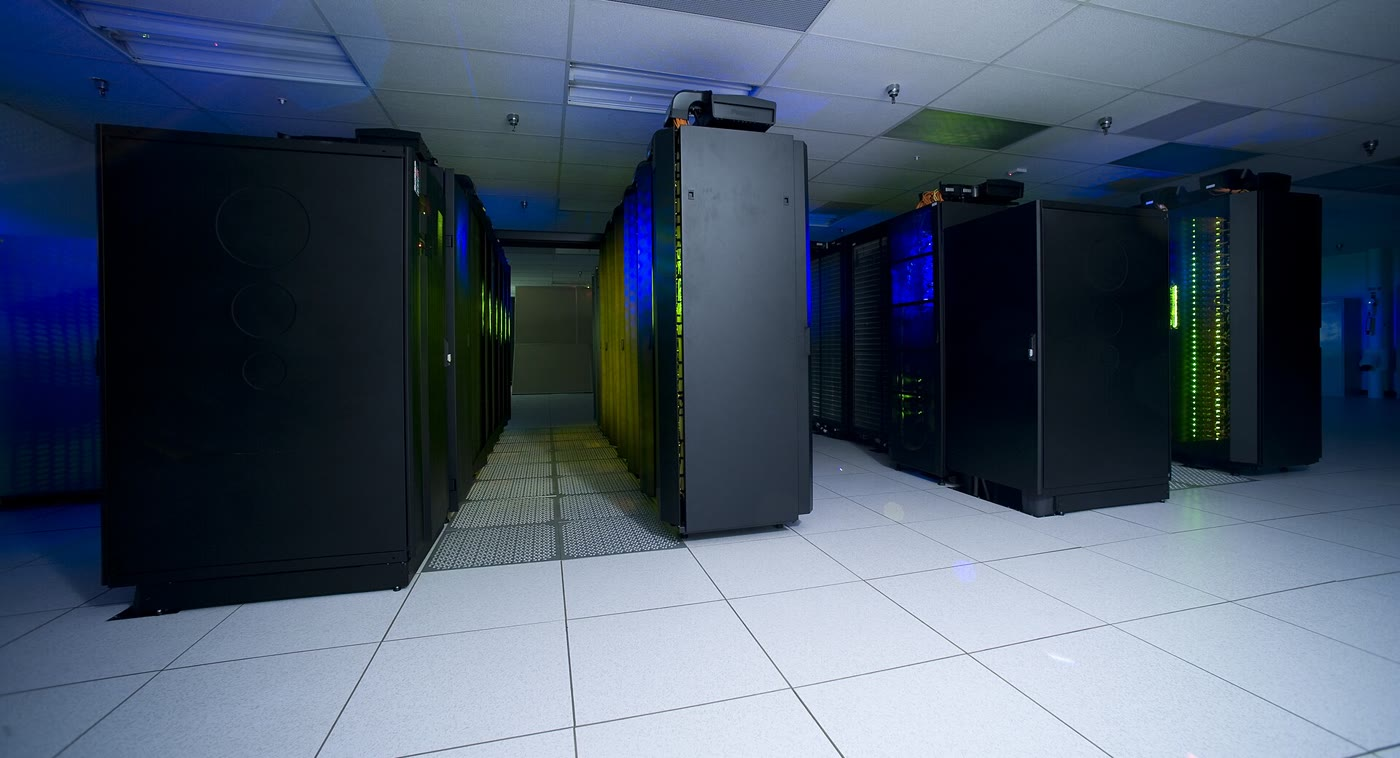
\includegraphics[width=0.7\linewidth]{images/book5/b3-nccs-supercomputer.jpg}

\par\smallskip{\small Bastidores de una supercomputadora del NASA Center for
Climate Simulation, Goddard Space Flight Center, en 2010 (NASA, dominio
público). Las ecuaciones de un modelo global se resuelven numéricamente en tales
ordenadores de alto rendimiento.}\label{fig:b3:climate-models:supercomputer}
\end{omfigure}
% ledger: photo:b3-nccs, ar6ch1:esm

\section{Evaluación de modelos}\label{sec:b3:climate-models:evaluation}

Un modelo se contrasta con el clima observado; el problema es que también se ha
ajustado a él. Cada \omterm{def:b3:climate-models:gcm}{parametrización} tiene parámetros cuyo
intervalo admisible viene fijado por la física y la observación, y a medida que se ensamblan los componentes
los modeladores los afinan hasta que el clima simulado cumple un
conjunto de objetivos de ajuste: el clima medio —por ejemplo, una temperatura media
cercana a la observada con la insolación de hoy—, los rasgos regionales o
las tendencias del periodo histórico. Solo entonces se libera el modelo para
las intercomparaciones.
% ledger: ar6ch1:models, ar6ch1:parameterization, ar6ch1:large-ensembles

\begin{definition}[Proyecto de intercomparación de modelos]\label{def:b3:climate-models:cmip}
Un \emph{proyecto de intercomparación de modelos}\index{proyecto de intercomparación de modelos}
es un conjunto coordinado de experimentos —los mismos forzamientos, los mismos
protocolos y las mismas salidas— ejecutados por numerosos grupos de modelización con
sus propios modelos, de modo que los resultados puedan compararse. El Coupled Model
Intercomparison Project (CMIP) se desarrolla en fases sucesivas; su sexta fase,
CMIP6, fue una línea clave de evidencia del sexto informe de evaluación.
\end{definition}

\begin{dated}{2021}
De los 29 grupos de modelización de CMIP6 que informaron de cómo ajustaron, 23 no
ajustaron su modelo al calentamiento observado durante el periodo histórico, y
25 no ajustaron su ECS: la sensibilidad de la mayoría de los modelos es una
propiedad emergente, no un dato de entrada. En promedio, los modelos de CMIP6 tienen una ECS y una TCR más altas que los
de la fase anterior, y una dispersión mayor que la de los rangos evaluados por el
informe; en algunos modelos esto se atribuyó a la retroalimentación de
las nubes de latitudes medias y altas. Algunos de los modelos más sensibles
reproducen peor el calentamiento reciente observado y los climas del pasado.
La evaluación no tomó, por tanto, sus rangos de ECS y TCR directamente de los
modelos, sino del conocimiento de los procesos de retroalimentación,
el registro instrumental, los climas del pasado y las restricciones emergentes; los trata como guía de
resultados de baja probabilidad y alto impacto (\emph{confianza alta}).
\end{dated}
% ledger: ar6ch1:models, ar6ch7:cmip6-sensitivity

\begin{definition}[Gran conjunto; restricción emergente]\label{def:b3:climate-models:evaluation}
Un \emph{gran conjunto}\index{gran conjunto} es un grupo de muchas simulaciones
de un único modelo, con los mismos forzamientos en el mismo periodo, que difieren
solo en sus estados iniciales. Una \emph{restricción
emergente}\index{restricción emergente} es una relación, hallada en un
conjunto de modelos distintos, entre una magnitud observable del
clima actual y una magnitud del futuro, como la ECS; el
valor observado de la primera acota entonces el rango de la segunda.
\end{definition}

El clima es caótico, de modo que diferencias mínimas del estado inicial llevan a los
miembros de un \omterm{def:b3:climate-models:evaluation}{gran conjunto} por trayectorias distintas: la dispersión de los
miembros mide la variabilidad interna, y su media, la respuesta
forzada. Los grandes conjuntos de varios modelos respaldaron la evaluación. Una
\omterm{def:b3:climate-models:evaluation}{restricción emergente} necesita una razón física. Con unas pocas decenas de modelos,
pueden probarse miles de observables, y algunos correlacionarán con la
ECS por azar; la evaluación conservó aquellos con base física, muchos de
ellos sobre las nubes de los trópicos, y advirtió de que un sesgo compartido por todos
los modelos del conjunto anula el método.
% ledger: ar6ch1:large-ensembles, ar6ch7:emergent

\begin{inthelab}[Un centro de modelización]
\begin{minipage}[t]{0.55\linewidth}\vspace{0pt}
En un centro de modelización climática, el modelo es un programa escrito y
mantenido por un equipo: la atmósfera, el océano, el hielo marino y la superficie
continental son componentes separados que intercambian flujos en sus interfaces a través de un acoplador. Antes
de cada ejecución se leen los forzamientos del experimento: las concentraciones de
gases de efecto invernadero, los aerosoles y los usos del suelo del protocolo. El globo se
divide en porciones que los procesadores del supercomputador calculan en paralelo,
y un siglo de clima modelado vuelve como un gran archivo de
campos. Los científicos los muestran en pantallas, los comparan con
reanálisis y registros de satélite, y envían las salidas estándar al
archivo de la intercomparación, donde otros grupos las comparan con las suyas.
\end{minipage}\hfill
\begin{minipage}[t]{0.42\linewidth}\vspace{0pt}
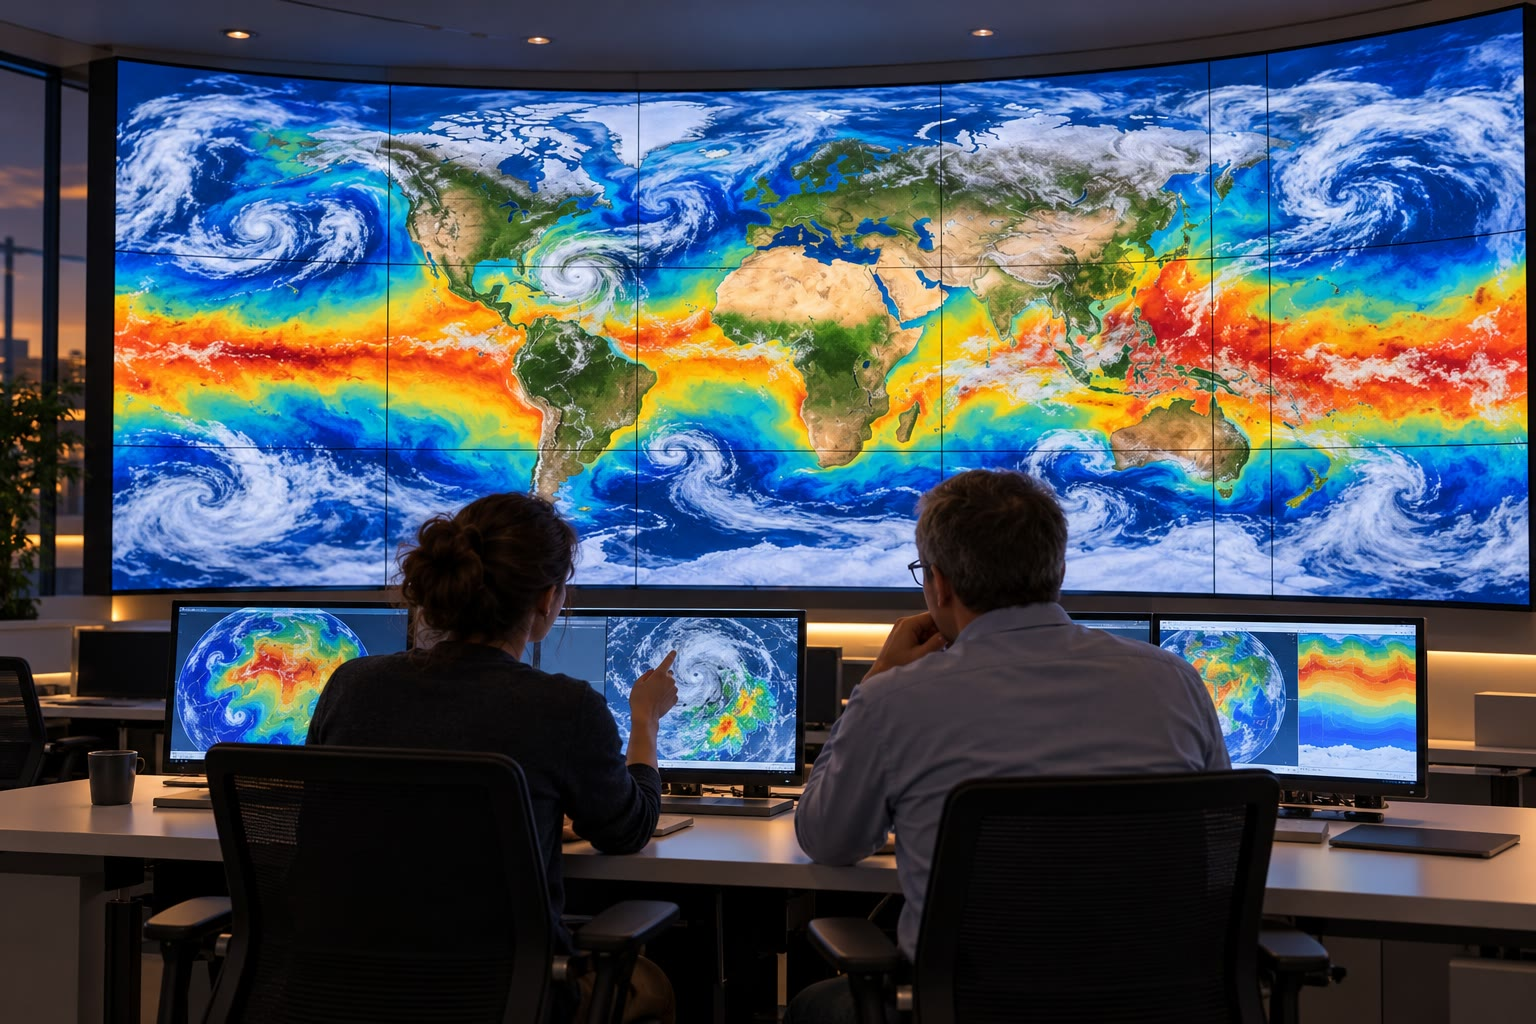
\includegraphics[width=\linewidth]{images/book5/ai/b3-model-centre.jpg}

{\scriptsize Dos científicos frente a una pared de pantallas que muestran campos globales
de una simulación de modelo. Ilustración generada por IA.}
\end{minipage}
\end{inthelab}
% ledger: ar6ch1:esm, ar6ch1:models

\section{Ejercicios}

\begin{exercise}[$\star$]\label{exo:b3:climate-models:1}
La ley de Budyko para la radiación de onda larga saliente es $I = a + bT - (a_1 + b_1T)n$, con $a = 14.0$, $b =
0.14$, $a_1 = 3.0$, $b_1 = 0.10$, en \unit{kcal.cm^{-2}} por mes y $T$
en \unit{\celsius}. Para una nubosidad $n = 0.5$, calcúlense $A$ y $B$, y
conviértanse a \unit{W/m^2} y \unit{W.m^{-2}.\celsius^{-1}}, tomando un mes
como una doceava parte de un año de 365.25 días. ¿Qué OLR da la ley a
\qty{15}{\celsius}?
\end{exercise}
% ledger: budyko69:olr

\begin{exercise}[$\star$]\label{exo:b3:climate-models:2}
Con $Q = \qty{340}{W/m^2}$, $A = \qty{211.9}{W/m^2}$ y $B =
\qty{1.816}{W.m^{-2}.\celsius^{-1}}$, calcúlese la temperatura de equilibrio
para un albedo de 0.30 y de 0.31. ¿Cuánto enfría este planeta un aumento de 0.01 del
albedo?
\end{exercise}

\begin{exercise}[$\star$]\label{exo:b3:climate-models:3}
Calcúlese la capacidad calorífica por metro cuadrado de una capa de mezcla de agua de mar
de \qty{60}{m} de profundidad, $\rho = \qty{1025}{kg/m^3}$ y $c_p = \qty{3992}{J.kg^{-1}.K^{-1}}$,
en \unit{J.m^{-2}.K^{-1}} y en \unit{W.yr.m^{-2}.K^{-1}}. Calcúlese el
tiempo de respuesta del \cref{thm:b3:climate-models:response} para $\lambda = -B =
\qty{-1.816}{W.m^{-2}.\celsius^{-1}}$ y para $\lambda =
\qty{-1.33}{W.m^{-2}.\celsius^{-1}}$.
\end{exercise}
% ledger: teos10:cp0

\begin{exercise}[$\star$]\label{exo:b3:climate-models:4}
Para el modelo de dos capas con $\lambda = \qty{-1.33}{W.m^{-2}.\celsius^{-1}}$,
$\gamma = \qty{0.62}{W.m^{-2}.\celsius^{-1}}$ y $F_{2\times} =
\qty{3.93}{W/m^2}$, calcúlense la ECS, la TCR aproximada $F_{2\times}/
(\gamma - \lambda)$, y su razón.
\end{exercise}
% ledger: ar6sm7:two-layer, ipcc:erf-2xco2

\begin{exercise}[$\star\star$]\label{exo:b3:climate-models:5}
En el modelo de cero dimensiones del texto, tómese una constante solar de
\qty{1340}{W/m^2}. Encuéntrense los tres equilibrios y la pendiente $N'(T)$ del
flujo neto en cada uno; ¿cuáles son estables?
\end{exercise}

\begin{exercise}[$\star\star$]\label{exo:b3:climate-models:6}
Modifíquese la rampa de albedo del texto: $\alpha = 0.62$ por debajo de \qty{-20}{\celsius},
$0.30$ por encima de \qty{0}{\celsius}, lineal entre ambos. Manténganse $A$ y $B$. ¿A qué
constante solar termina la rama cálida, y en cuántos por ciento queda esa
por debajo de \qty{1360}{W/m^2}? ¿A qué constante solar se funde la bola de nieve?
¿Qué fija el tamaño del umbral?
\end{exercise}

\begin{exercise}[$\star\star$]\label{exo:b3:climate-models:7}
Un planeta modelo con los parámetros del texto está en el estado de bola de nieve.
(a)~¿Cuál es su temperatura con la constante solar actual? (b)~Manteniendo el Sol
tal como está, ¿qué forzamiento $F$ llevaría la temperatura de la bola de nieve hasta
\qty{-10}{\celsius}? ¿Cuántas veces es el forzamiento de una duplicación del dióxido de carbono,
\qty{3.93}{W/m^2}? (c)~Una vez desaparecido el hielo, ¿dónde se asienta el planeta
si después se retira el forzamiento?
\end{exercise}
% ledger: ipcc:erf-2xco2, hoffman17:hysteresis

\begin{exercise}[$\star\star$]\label{exo:b3:climate-models:8}
El modelo X, un modelo de dos capas inventado, tiene $C = 7.0$ y $C_d =
\qty{90}{W.yr.m^{-2}.\celsius^{-1}}$, $\gamma = 0.70$ y $\lambda =
\qty{-1.10}{W.m^{-2}.\celsius^{-1}}$. Calcúlense sus dos escalas de tiempo exactamente
y con las aproximaciones del \cref{thm:b3:climate-models:two-layer}, la
fracción $a_f$, su ECS y su TCR aproximada.
\end{exercise}

\begin{exercise}[$\star\star$]\label{exo:b3:climate-models:9}
En el modelo de Budyko del texto, $\bar T = \qty{12.81}{\celsius}$, $\beta =
\qty{3.74}{W.m^{-2}.\celsius^{-1}}$, la línea de hielo en \ang{72}, $s = 1.221$
en el ecuador y $0.506$ en el polo, $\alpha = 0.30$ y $0.62$.
Calcúlense la temperatura en el ecuador y en el polo, y el calor
$\beta(T - \bar T)$ que el transporte extrae de, o aporta a, cada
metro cuadrado allí.
\end{exercise}

\begin{exercise}[$\star\star\star$]\label{exo:b3:climate-models:10}
Un planeta sin hielo ($\alpha = 0.30$ en todas partes) tiene el transporte difusivo
$D = -\mathcal D\,\partial_x[(1 - x^2)\partial_xT]$ y la
insolación $s(x) = 1 + s_2P_2(x)$, $P_2 = (3x^2 - 1)/2$. (a)~Muéstrese que
$\partial_x[(1 - x^2)\partial_xP_2] = -6P_2$. (b)~Muéstrese que $T = T_0 +
T_2P_2(x)$ es una solución estacionaria, con $T_0 = (Q(1 - \alpha) - A)/B$ y
$T_2 = Qs_2(1 - \alpha)/(B + 6\mathcal D)$. (c)~La insolación de la
reanálisis da $s_2 = \num{-0.476}$. Sin transporte, ¿cuál sería la
diferencia de temperatura entre el ecuador y el polo? (d)~¿Qué $\mathcal D$ da
la diferencia observada, \qty{55.3}{\celsius}?
\end{exercise}
% ledger: data:b3-ncep, data:b5-ncep-air

\begin{exercise}[$\star\star\star$]\label{exo:b3:climate-models:11}
(a)~Escríbase la cuadrática del \cref{thm:b3:climate-models:two-layer} como $r^2 -
\Sigma r + \Pi = 0$ y muéstrese que, si $4\Pi \ll \Sigma^2$, sus raíces son
próximas a $\Sigma$ y $\Pi/\Sigma$. (b)~Para un forzamiento $F = kt$ que crece
linealmente, muéstrese que una vez $t \gg \tau_f$, y mientras $T_d$ se mantenga pequeño,
$T \approx kt/(\gamma - \lambda)$; dedúzcase la TCR aproximada. (c)~Compruébense
los números del texto: $\Sigma$, $\Pi$, las dos escalas de tiempo y la
razón $4\Pi/\Sigma^2$.
\end{exercise}
% ledger: ar6sm7:two-layer

\begin{exercise}[$\star\star\star$]\label{exo:b3:climate-models:12}
Un conjunto inventado de ocho modelos proporciona un observable $X$ del
clima actual y su ECS:
\begin{center}
\begin{tabular}{l*{8}{c}}
\hline
$X$ & 0.2 & 0.5 & 0.6 & 0.8 & 1.0 & 1.1 & 1.3 & 1.5\\
ECS (\unit{\celsius}) & 2.3 & 2.7 & 3.1 & 3.2 & 3.8 & 3.9 & 4.4 & 4.6\\
\hline
\end{tabular}
\end{center}
(a)~Calcúlense la media y la desviación típica de la ECS del
conjunto. (b)~Ajústese la ECS $= a + bX$ por mínimos cuadrados; calcúlense la correlación
y la desviación típica de los residuos. (c)~La $X$ observada es $0.7
\pm 0.1$. ¿Qué ECS da la restricción y con qué dispersión?
(d)~¿Qué haría desconfiar de esta restricción?
\end{exercise}
% ledger: ar6ch7:emergent

\section{Problema: ¿qué tan cerca de una bola de nieve?}

\begin{problem}[{Problema de fin de semana --- equilibrios, estabilidad y el
umbral de glaciación de un planeta modelo}]
\label{pb:b3:climate-models:1}
Un planeta modelo tiene la constante solar actual $S_0 = \qty{1360}{W/m^2}$ y el
ley de OLR $A + BT$ con $A = \qty{211.9}{W/m^2}$ y $B =
\qty{1.816}{W.m^{-2}.\celsius^{-1}}$. Su albedo es 0.62 por debajo de
\qty{-10}{\celsius}, 0.30 por encima de \qty{+10}{\celsius}, con variación lineal entre ambos, y
su capacidad calorífica superficial $C = \qty{8.1}{W.yr.m^{-2}.\celsius^{-1}}$. Tómese
$\sigma = \qty{5.670e-8}{W.m^{-2}.K^{-4}}$.

\medskip\noindent\textbf{Parte I --- El planeta en equilibrio.}
\begin{enumerate}
\item Calcúlese la insolación media $Q_0$ por metro cuadrado del planeta, y
  explíquese el factor.
\item Calcúlense la insolación absorbida con un albedo de 0.30, y la OLR a
  \qty{15}{\celsius}.
\item Calcúlese el equilibrio cálido.
\item Calcúlese el equilibrio de bola de nieve, y compruébese que se sitúa en la
  rama helada.
\item Calcúlese el tercer equilibrio, sobre la rampa de albedo.
\item Calcúlese la temperatura de emisión que devuelve al espacio, como cuerpo negro,
  la insolación absorbida, y compárese con el equilibrio cálido.
\end{enumerate}

\medskip\noindent\textbf{Parte II --- Estabilidad y tiempo.}
\begin{enumerate}[resume]
\item Calcúlese la pendiente $N'(T)$ del flujo neto en cada equilibrio, y díganse
  cuáles son estables.
\item Una pequeña desviación respecto del equilibrio intermedio crece como $\mathrm
  e^{t/\tau}$. Calcúlese $\tau$.
\item Calcúlese el tiempo de respuesta del equilibrio cálido.
\item Un forzamiento de \qty{3.93}{W/m^2}, el de duplicar el dióxido de carbono,
  se activa. Calcúlese el calentamiento en equilibrio y compárese con
  la ECS evaluada para el clima real.
\item ¿Cuánto tarda el modelo en alcanzar el \qty{95}{\percent} del
  calentamiento? ¿Por qué tarda más el clima real?
\end{enumerate}

\medskip\noindent\textbf{Parte III --- La bifurcación silla-nodo.}
\begin{enumerate}[resume]
\item A medida que el Sol se atenúa, ¿a qué temperatura el equilibrio cálido
  se encuentra con el intermedio? Calcúlese $Q$ allí.
\item Calcúlese la constante solar en la bifurcación, y la caída
  respecto de hoy, en tanto por ciento.
\item Justo por debajo, ¿a dónde va el clima? Calcúlese su temperatura.
\item Calcúlese la constante solar a la que se funde la bola de nieve, y el aumento
  respecto de hoy, en tanto por ciento.
\item Dibújese el bucle que sigue la temperatura cuando $S_0$ se reduce
  por debajo de la bifurcación y después se restablece en \qty{1360}{W/m^2}.
\end{enumerate}

\medskip\noindent\textbf{Parte IV --- La línea de hielo.} Aplíquese al planeta
el modelo latitudinal de Budyko, con $\beta = \qty{3.739}{W.m^{-2}.\celsius^{-1}}$,
un albedo de hielo de 0.62 al polo de la línea de hielo, 0.30 hacia el ecuador, 0.50 en
el borde, y la insolación del reanálisis:
\begin{center}
\begin{tabular}{lccccccc}
\hline
latitud & \ang{0} & \ang{30} & \ang{40} & \ang{47.5} & \ang{55} & \ang{60} & \ang{72}\\
$s(x_s)$ & 1.2211 & 1.0730 & 0.9647 & 0.8688 & 0.7650 & 0.6947 & 0.5643\\
$F(x_s)$ & 0 & 0.5865 & 0.7324 & 0.8192 & 0.8863 & 0.9205 & 0.9738\\
\hline
\end{tabular}
\end{center}
\begin{enumerate}[resume]
\item Con la línea de hielo en \ang{72}, calcúlense el albedo medio $\bar\alpha$
  y la temperatura media $\bar T$.
\item Calcúlese la temperatura crítica $T_c$ que sitúa el borde en
  \ang{72} hoy, y compárese con el reanálisis, \qty{-15.8}{\celsius}.
\item Calcúlese el numerador de $Q(x_s)$ en la \cref{prop:b3:climate-models:iceline}
  y la razón $\beta/B$.
\item Calcúlese $Q(x_s)/Q_0$ para la línea de hielo en \ang{30}, \ang{40},
  \ang{47.5}, \ang{55} y \ang{60}.
\item ¿Dónde está el mínimo de estos valores? ¿Qué líneas de hielo son estables?
\item ¿Con el Sol actual, qué otra línea de hielo admite el modelo, y es
  estable? ¿Es posible hoy la bola de nieve? (Úsese la columna \ang{0}.)
\item Compárese el umbral del modelo latitudinal con el de la Parte~III
  y con el \qty{1.6}{\percent} de Budyko, y la latitud del hielo en el
  umbral con la suya, \ang{50}.
\item Dése, con dos cifras significativas, la caída de la constante solar, en
  tanto por ciento, que lleva al planeta modelo a la glaciación.
\end{enumerate}
\end{problem}
% ledger: nasa:solar-mean, data:b5-ncep-air, data:b3-ncep, budyko69:transport, budyko69:albedo, budyko69:threshold, ipcc:ecs, const:sigma
